\documentclass{article}

\usepackage{graphicx}
\usepackage{caption}
\usepackage{subcaption}

\renewcommand{\figurename}{Slika}

\title{NENR - 6. domaća zadaća: ANFIS}
\author{Mate Gašparini}
\date{Zagreb, prosinac, 2019.}

\begin{document}

\maketitle

\section{Izvod pravila učenja}

\begin{itemize}
    \item izlaz sustava za $k$-ti uzorak:
    $ o_k = \frac{\sum_{j = 1}^{m}{w_j z_j}}{\sum_{j = 1}^{m}{w_j}} $,
    $ w_i = A_i(x) B_i(y) $
    \item funkcija pripadnosti:
    $ A(x) = \sigma(x) = \frac{1}{1 + e^{b(x - a)}} $
    \item pogreška uzorka:
    $ E_k = \frac{1}{2} (t_k - o_k)^2 $
    \item ažuriranje parametra $ \psi $ (općenito):
    $ \psi(t + 1) = \psi(t) - \eta \frac{\partial E_k}{\partial \psi} $
\end{itemize}

\subsection{Pomoćne parcijalne derivacije}

\begin{equation}
    \frac{\partial E_k}{\partial o_k} =
    \frac{1}{2} 2 (t_k - o_k) (-1) =
    - (t_k - o_k)
\end{equation}
\begin{equation}
    \frac{\partial o_k}{\partial w_i} =
    \frac{\sum_{j = 1}^{m}{w_j (z_i - z_j)}}{(\sum_{j = 1}^{m}{w_j})^2}
\end{equation}
\begin{equation}
    \frac{\partial o_k}{\partial z_i} =
    \frac{w_i}{\sum_{j = 1}^{m}{w_j}}
\end{equation}
\begin{equation}
    \frac{\partial \sigma}{\partial x} =
    \sigma(x) (1 - \sigma(x))
\end{equation}

\subsection{Ažuriranje parametra $ a_i $}

\begin{equation}
    \frac{\partial E_k}{\partial a_i} =
    \frac{\partial E_k}{\partial o_k} \frac{\partial o_k}{\partial w_i} \frac{\partial w_i}{\partial a_i}
\end{equation}
\begin{equation}
    \frac{\partial w_i}{\partial a_i} =
    B_i(y) A_i(x)(1 - A_i(x)) b_i
\end{equation}
\begin{equation}
    \frac{\partial E_k}{\partial a_i} =
    - (t_k - o_k) \frac{\sum_{j = 1}^{m}{w_j (z_i - z_j)}}{(\sum_{j = 1}^{m}{w_j})^2} A_i(x)(1 - A_i(x)) B_i(y) b_i
\end{equation}

\subsection{Ažuriranje parametra $ b_i $}

\begin{equation}
    \frac{\partial E_k}{\partial b_i} =
    \frac{\partial E_k}{\partial o_k} \frac{\partial o_k}{\partial w_i} \frac{\partial w_i}{\partial b_i}
\end{equation}
\begin{equation}
    \frac{\partial w_i}{\partial b_i} =
    B_i(y) A_i(x)(1 - A_i(x)) (a_i - x)
\end{equation}
\begin{equation}
    \frac{\partial E_k}{\partial b_i} =
    - (t_k - o_k) \frac{\sum_{j = 1}^{m}{w_j (z_i - z_j)}}{(\sum_{j = 1}^{m}{w_j})^2} A_i(x)(1 - A_i(x)) B_i(y) (a_i - x)
\end{equation}

\subsection{Ažuriranje parametra $ c_i $}

\begin{equation}
    \frac{\partial E_k}{\partial c_i} =
    \frac{\partial E_k}{\partial o_k} \frac{\partial o_k}{\partial w_i} \frac{\partial w_i}{\partial c_i}
\end{equation}
\begin{equation}
    \frac{\partial w_i}{\partial c_i} =
    A_i(x) B_i(y)(1 - B_i(y)) d_i
\end{equation}
\begin{equation}
    \frac{\partial E_k}{\partial c_i} =
    - (t_k - o_k) \frac{\sum_{j = 1}^{m}{w_j (z_i - z_j)}}{(\sum_{j = 1}^{m}{w_j})^2} A_i(x) B_i(y)(1 - B_i(y)) d_i
\end{equation}

\subsection{Ažuriranje parametra $ d_i $}

\begin{equation}
    \frac{\partial E_k}{\partial d_i} =
    \frac{\partial E_k}{\partial o_k} \frac{\partial o_k}{\partial w_i} \frac{\partial w_i}{\partial d_i}
\end{equation}
\begin{equation}
    \frac{\partial w_i}{\partial d_i} =
    A_i(x) B_i(y)(1 - B_i(y)) (c_i - y)
\end{equation}
\begin{equation}
    \frac{\partial E_k}{\partial d_i} =
    - (t_k - o_k) \frac{\sum_{j = 1}^{m}{w_j (z_i - z_j)}}{(\sum_{j = 1}^{m}{w_j})^2} A_i(x) B_i(y)(1 - B_i(y)) (c_i - y)
\end{equation}

\subsection{Ažuriranje parametra $ p_i $}

\begin{equation}
    \frac{\partial E_k}{\partial p_i} =
    \frac{\partial E_k}{\partial o_k} \frac{\partial o_k}{\partial z_i} \frac{\partial z_i}{\partial p_i}
\end{equation}
\begin{equation}
    \frac{\partial z_i}{\partial p_i} =
    x
\end{equation}
\begin{equation}
    \frac{\partial E_k}{\partial p_i} =
    - (t_k - o_k) \frac{w_i}{\sum_{j = 1}^{m}{w_j}} x
\end{equation}

\subsection{Ažuriranje parametra $ q_i $}

\begin{equation}
    \frac{\partial E_k}{\partial q_i} =
    \frac{\partial E_k}{\partial o_k} \frac{\partial o_k}{\partial z_i} \frac{\partial z_i}{\partial q_i}
\end{equation}
\begin{equation}
    \frac{\partial z_i}{\partial q_i} =
    y
\end{equation}
\begin{equation}
    \frac{\partial E_k}{\partial p_i} =
    - (t_k - o_k) \frac{w_i}{\sum_{j = 1}^{m}{w_j}} y
\end{equation}

\subsection{Ažuriranje parametra $ r_i $}

\begin{equation}
    \frac{\partial E_k}{\partial r_i} =
    \frac{\partial E_k}{\partial o_k} \frac{\partial o_k}{\partial z_i} \frac{\partial z_i}{\partial r_i}
\end{equation}
\begin{equation}
    \frac{\partial z_i}{\partial r_i} =
    1
\end{equation}
\begin{equation}
    \frac{\partial E_k}{\partial r_i} =
    - (t_k - o_k) \frac{w_i}{\sum_{j = 1}^{m}{w_j}}
\end{equation}

\section{Varijante algoritma}

\begin{itemize}
    \item grupni gradijentni spust -
    ažuriranje parametara nakon izračuna sume gradijenata po svim uzorcima
    \item stohastički gradijentni spust -
    ažuriranje parametara nakon izračuna gradijenata za $k$-ti uzorak
\end{itemize}

\section{Primjeri za učenje}

\begin{figure}[h]
    \centering
    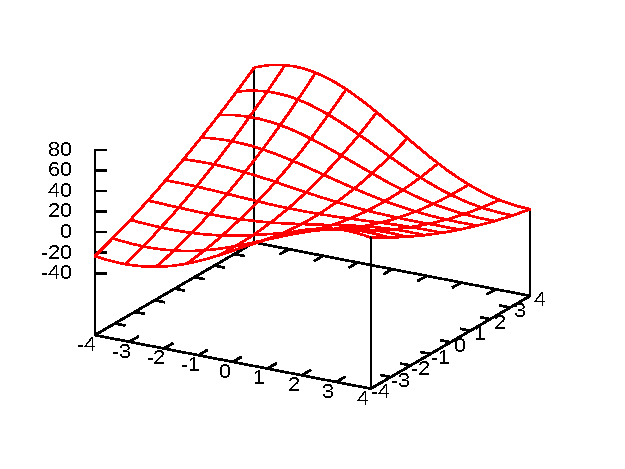
\includegraphics{img/dataset-function.pdf}
    \caption{Funkcija $ ((x - 1)^2 + (y + 2)^2 - 5 x y + 3) * cos^2(\frac{x}{5}) $}
\end{figure}

\begin{figure}[h]
    \centering
    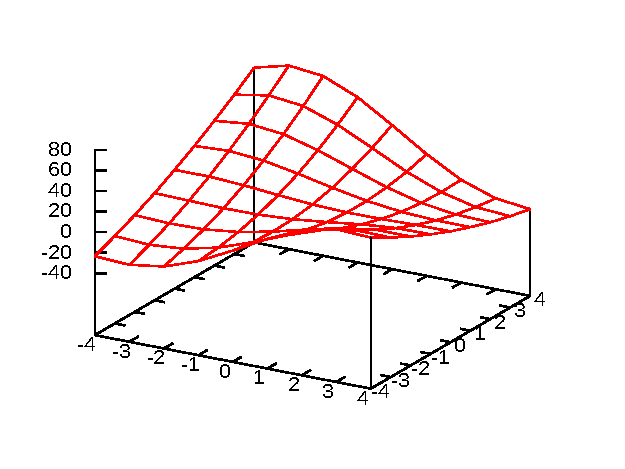
\includegraphics{img/dataset-sampled.pdf}
    \caption{Skup primjera za učenje generiran na intervalu $ [-4, 4] \times [-4, 4] \subset Z \times Z $ }
\end{figure}

\section{Provedeni postupci učenja}

Provedeni su postupci učenja za sustav od jedno, dva i pet pravila.
U svim postupcima korišteni su jednaki parametri:
\begin{itemize}
    \item broj epoha (10 000),
    \item stopa učenja parametara antecedenata (1e-5) te
    \item stopa učenja parametara konzekventa (1e-3).
\end{itemize}

Na slikama \ref{pred-1}, \ref{pred-2} i \ref{pred-5}
prikazane su naučene funkcije,
a na slikama \ref{err-1}, \ref{err-2} i \ref{err-5}
njihova odgovarajuća odstupanja od skupa primjera za učenje.
Porastom broja pravila, raste ekspresivnost i točnost sustava,
a padaju iznosi pogreške uzorka.

\begin{figure}[h]
    \centering
    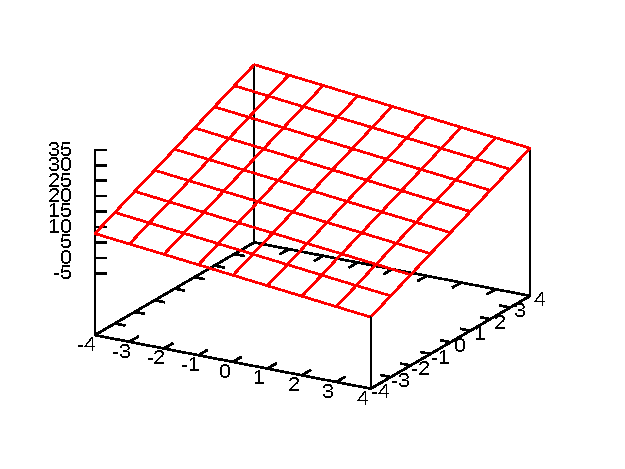
\includegraphics{img/prediction-batch-1.pdf}
    \caption{Naučena funkcija u sustavu s jednim pravilom}
    \label{pred-1}
\end{figure}

\begin{figure}[h]
    \centering
    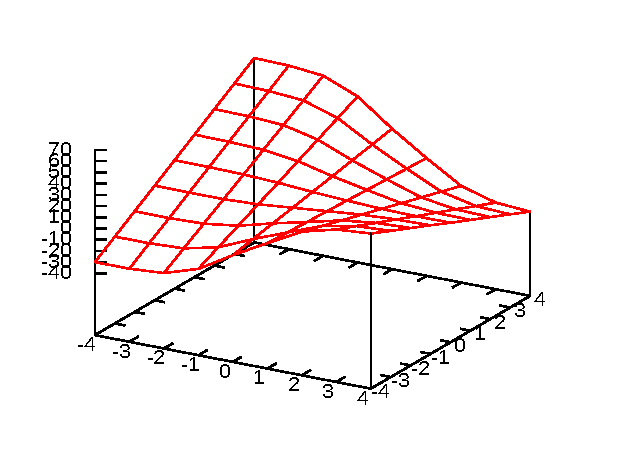
\includegraphics{img/prediction-batch-2.pdf}
    \caption{Naučena funkcija u sustavu s dvama pravilima}
    \label{pred-2}
\end{figure}

\begin{figure}[h]
    \centering
    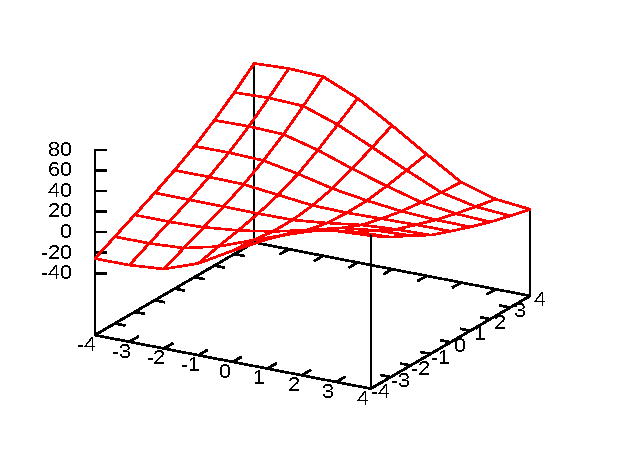
\includegraphics{img/prediction-batch-5.pdf}
    \caption{Naučena funkcija u sustavu s pet pravila}
    \label{pred-5}
\end{figure}

\begin{figure}[h]
    \centering
    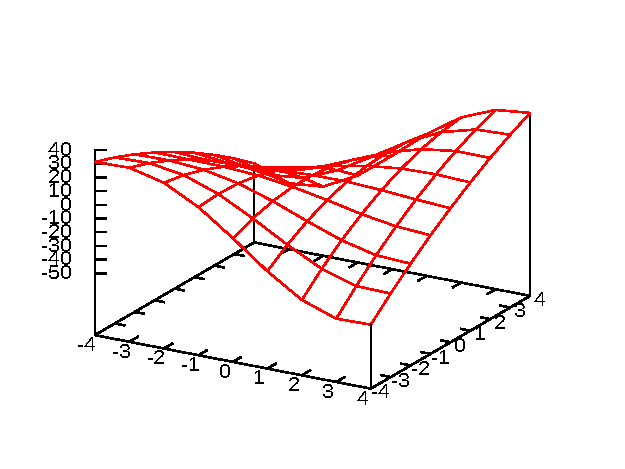
\includegraphics{img/errors-batch-1.pdf}
    \caption{Pogreška $ \delta $ u sustavu s jednim pravilom}
    \label{err-1}
\end{figure}

\begin{figure}[h]
    \centering
    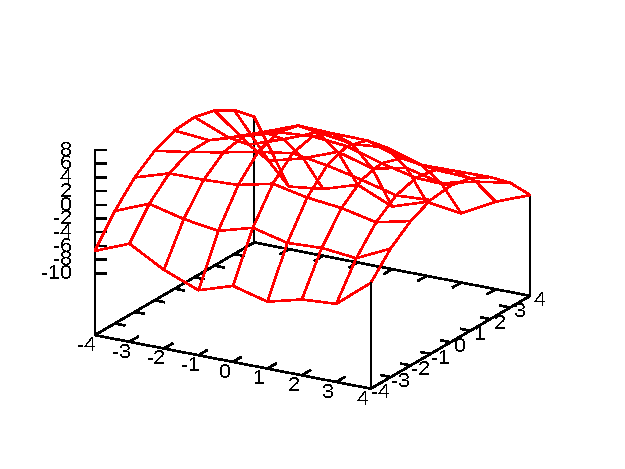
\includegraphics{img/errors-batch-2.pdf}
    \caption{Pogreška $ \delta $ u sustavu s dvama pravilima}
    \label{err-2}
\end{figure}

\begin{figure}[h]
    \centering
    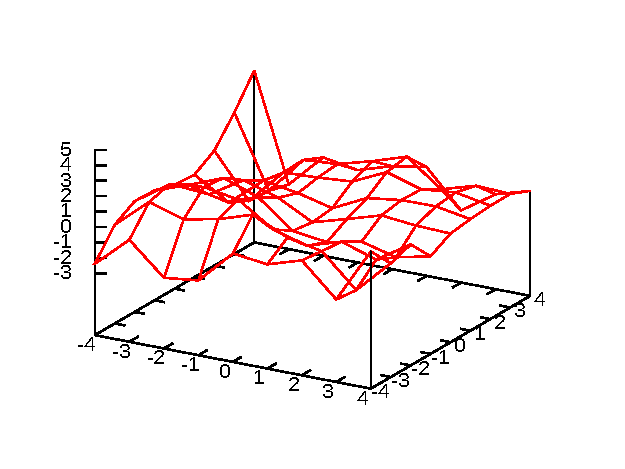
\includegraphics{img/errors-batch-5.pdf}
    \caption{Pogreška $ \delta $ u sustavu s pet pravila}
    \label{err-5}
\end{figure}

\subsection{Kretanje pogreške kroz epohe}

Na slikama \ref{mse-1}, \ref{mse-2} i \ref{mse-5}
prikazano je kretanje srednje kvadratne pogreške po epohama
za postupke učenja sustava sa jednim, dva i pet pravila.
Za svaki od postupaka učenja prikazana su dva grafa -
jedan za grupni, a drugi za stohastički postupak učenja.

\begin{figure}[h]
    \centering
    \begin{subfigure}[b]{0.49\textwidth}
        \centering
        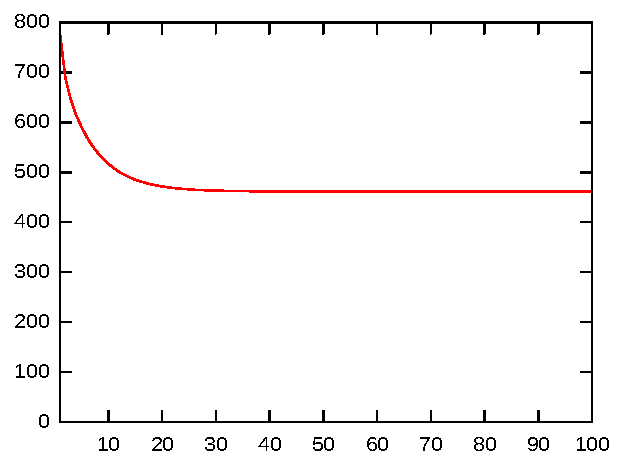
\includegraphics[width=\textwidth]{img/mse-batch-1.pdf}
        \caption{grupni postupak}
    \end{subfigure}
    \hfill
    \begin{subfigure}[b]{0.49\textwidth}
        \centering
        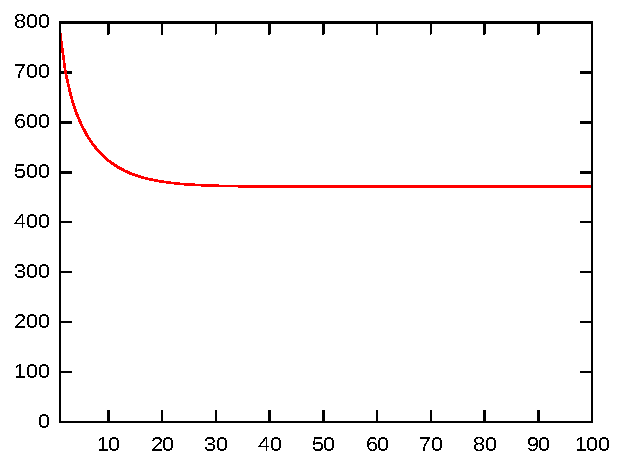
\includegraphics[width=\textwidth]{img/mse-stochastic-1.pdf}
        \caption{stohastički postupak}
    \end{subfigure}
    \hfill
    \caption{Kretanje srednje pogreške u sustavu s jednim pravilom}
    \label{mse-1}
\end{figure}

\begin{figure}[h]
    \centering
    \begin{subfigure}[b]{0.49\textwidth}
        \centering
        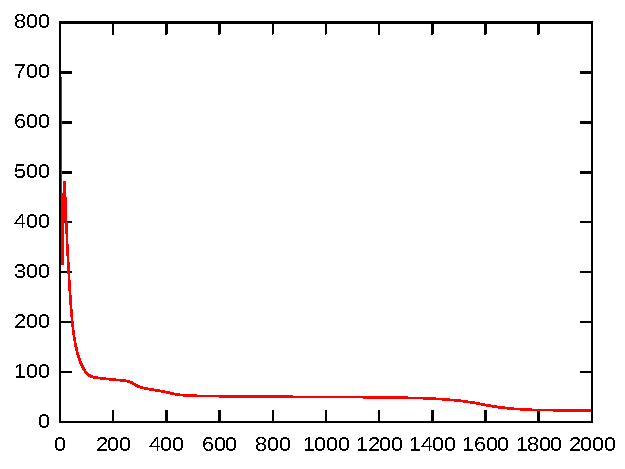
\includegraphics[width=\textwidth]{img/mse-batch-2.pdf}
        \caption{grupni postupak}
    \end{subfigure}
    \hfill
    \begin{subfigure}[b]{0.49\textwidth}
        \centering
        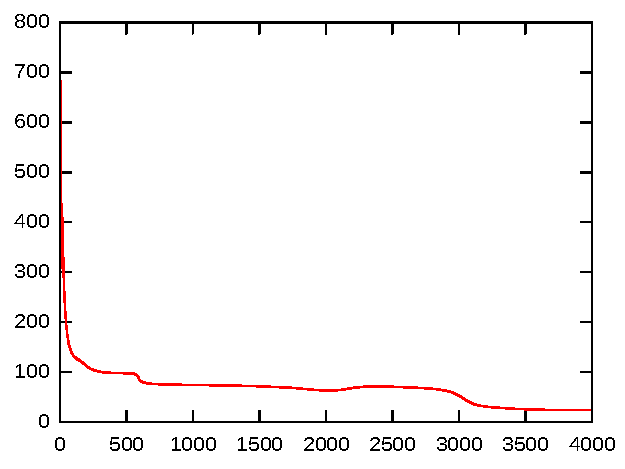
\includegraphics[width=\textwidth]{img/mse-stochastic-2.pdf}
        \caption{stohastički postupak}
    \end{subfigure}
    \hfill
    \caption{Kretanje srednje pogreške u sustavu s dvama pravilima}
    \label{mse-2}
\end{figure}

\begin{figure}[h]
    \centering
    \begin{subfigure}[b]{0.49\textwidth}
        \centering
        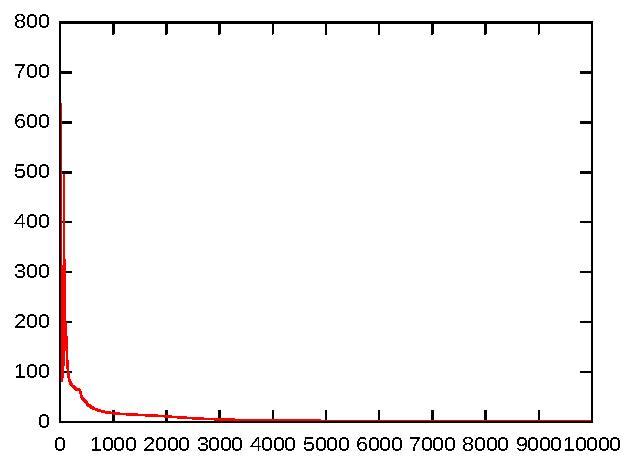
\includegraphics[width=\textwidth]{img/mse-batch-5.pdf}
        \caption{grupni postupak}
    \end{subfigure}
    \hfill
    \begin{subfigure}[b]{0.49\textwidth}
        \centering
        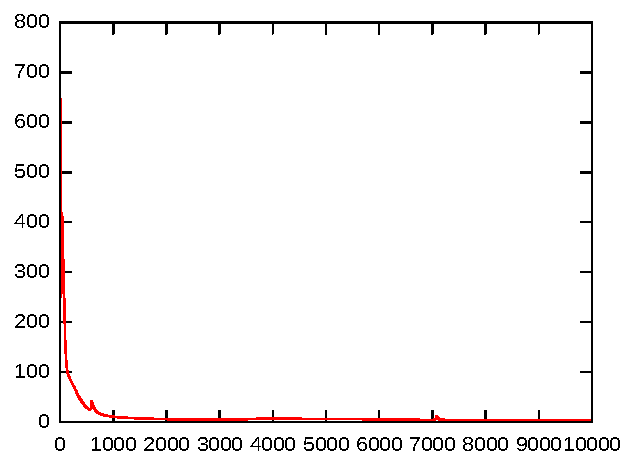
\includegraphics[width=\textwidth]{img/mse-stochastic-5.pdf}
        \caption{stohastički postupak}
    \end{subfigure}
    \hfill
    \caption{Kretanje srednje pogreške u sustavu s pet pravila}
    \label{mse-5}
\end{figure}

\section{Interpretacija pravila}

Na slikama \ref{rule-1}, \ref{rule-2}, \ref{rule-3}, \ref{rule-4} i \ref{rule-5}
prikazane su funkcije pripadnosti neizrazitih skupova $A$ i $B$
te su dane njihove moguće interpretacije.

\begin{figure}[h]
    \centering
    \begin{subfigure}[b]{0.49\textwidth}
        \centering
        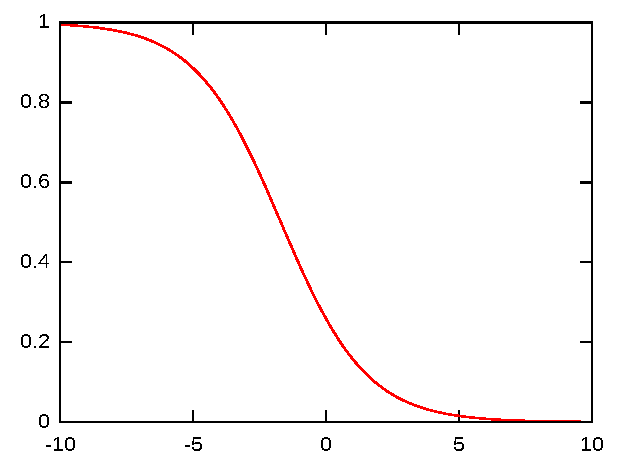
\includegraphics[width=\textwidth]{img/rule-1-A.pdf}
        \caption{$ a \approx -1.70 $, $ b \approx 0.62 $}
    \end{subfigure}
    \hfill
    \begin{subfigure}[b]{0.49\textwidth}
        \centering
        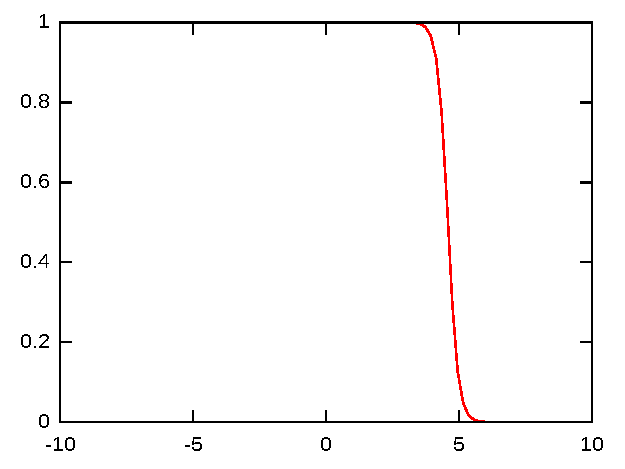
\includegraphics[width=\textwidth]{img/rule-1-B.pdf}
        \caption{$ a \approx 4.58 $, $ b \approx 5.22 $}
    \end{subfigure}
    \hfill
    \caption{Pravilo 1 - \textit{ako x je dosta manji od 5 i y je otprilike manji od 5}}
    \label{rule-1}
\end{figure}

\begin{figure}[h]
    \centering
    \begin{subfigure}[b]{0.49\textwidth}
        \centering
        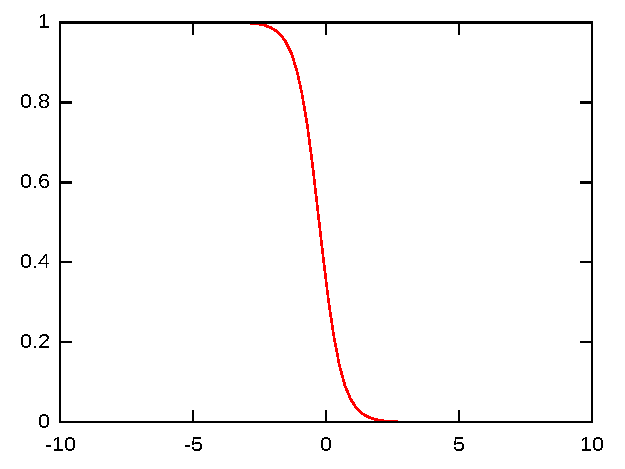
\includegraphics[width=\textwidth]{img/rule-2-A.pdf}
        \caption{$ a \approx -0.26 $, $ b \approx 2.36 $}
    \end{subfigure}
    \hfill
    \begin{subfigure}[b]{0.49\textwidth}
        \centering
        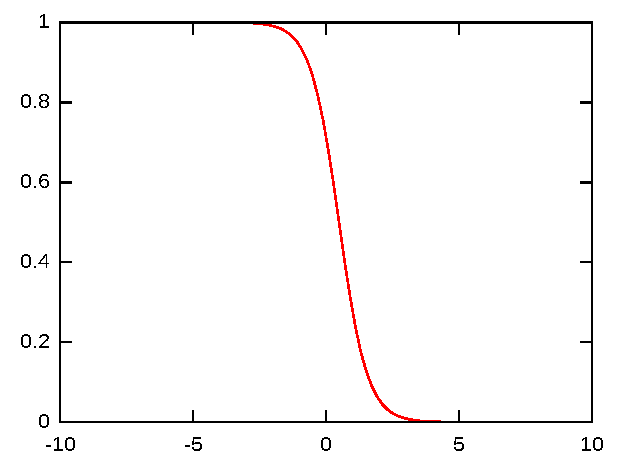
\includegraphics[width=\textwidth]{img/rule-2-B.pdf}
        \caption{$ a \approx 0.49 $, $ b \approx 1.88 $}
    \end{subfigure}
    \hfill
    \caption{Pravilo 2 - \textit{ako x je otprilike negativan i y je otprilike negativan}}
    \label{rule-2}
\end{figure}

\begin{figure}[h]
    \centering
    \begin{subfigure}[b]{0.49\textwidth}
        \centering
        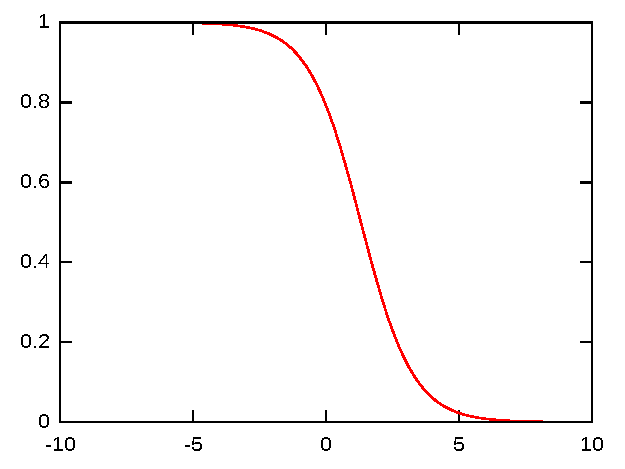
\includegraphics[width=\textwidth]{img/rule-3-A.pdf}
        \caption{$ a \approx 1.31 $, $ b \approx 1.02 $}
    \end{subfigure}
    \hfill
    \begin{subfigure}[b]{0.49\textwidth}
        \centering
        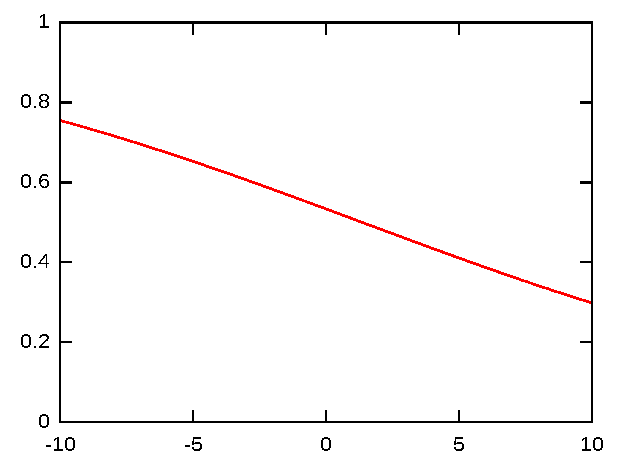
\includegraphics[width=\textwidth]{img/rule-3-B.pdf}
        \caption{$ a \approx 1.34 $, $ b \approx 0.10 $}
    \end{subfigure}
    \hfill
    \caption{Pravilo 3 - \textit{ako x je dosta manji od 5 i y je dosta manji od 30}}
    \label{rule-3}
\end{figure}

\begin{figure}[h]
    \centering
    \begin{subfigure}[b]{0.49\textwidth}
        \centering
        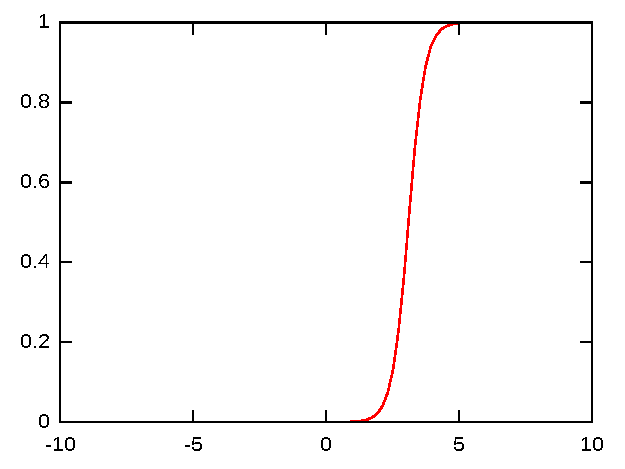
\includegraphics[width=\textwidth]{img/rule-4-A.pdf}
        \caption{$ a \approx 3.10 $, $ b \approx -3.25 $}
    \end{subfigure}
    \hfill
    \begin{subfigure}[b]{0.49\textwidth}
        \centering
        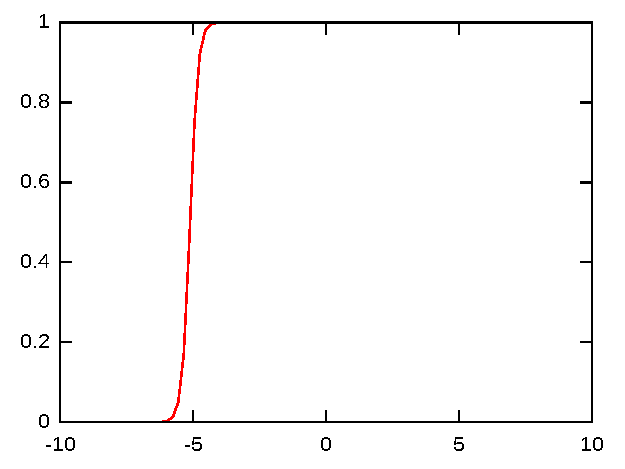
\includegraphics[width=\textwidth]{img/rule-4-B.pdf}
        \caption{$ a \approx -5.12 $, $ b \approx -6.69 $}
    \end{subfigure}
    \hfill
    \caption{Pravilo 4 - \textit{ako x je otprilike veći od 3 i y je otprilike veći od -5}}
    \label{rule-4}
\end{figure}

\begin{figure}[h]
    \centering
    \begin{subfigure}[b]{0.49\textwidth}
        \centering
        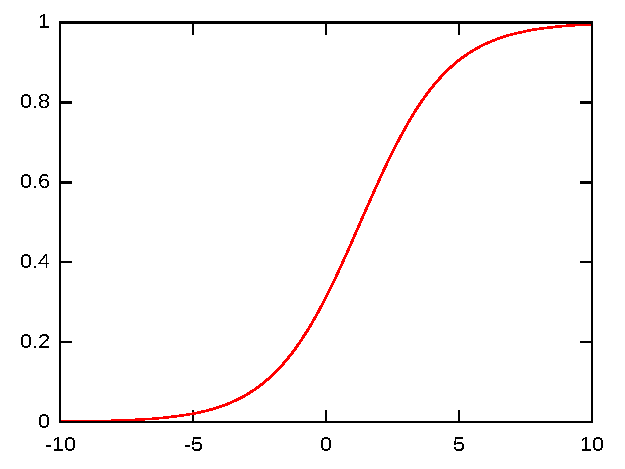
\includegraphics[width=\textwidth]{img/rule-5-A.pdf}
        \caption{$ a \approx 1.29 $, $ b \approx -0.61 $}
    \end{subfigure}
    \hfill
    \begin{subfigure}[b]{0.49\textwidth}
        \centering
        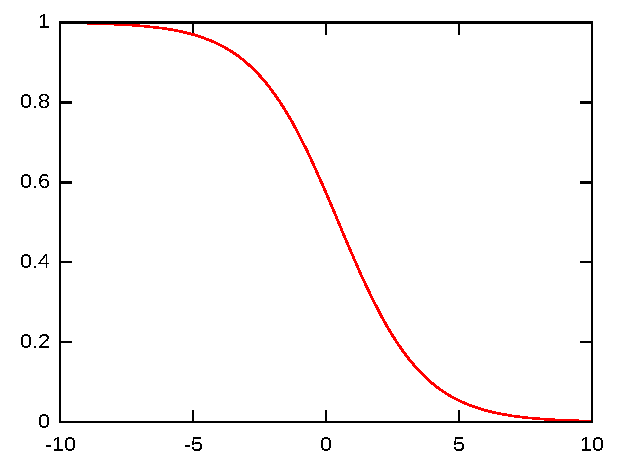
\includegraphics[width=\textwidth]{img/rule-5-B.pdf}
        \caption{$ a \approx 0.46 $, $ b \approx 0.63 $}
    \end{subfigure}
    \hfill
    \caption{Pravilo 5 - \textit{ako x je dosta veći od -5 i y je dosta manji od 5}}
    \label{rule-5}
\end{figure}

\section{Odabir stope učenja}

Na slici \ref{eta-batch} prikazano je kretanje srednje kvadratne pogreške
prilikom grupnog postupka učenja za:
\begin{itemize}
    \item premalu ($ \eta_a =$ 1e-8, $ \eta_c =$ 1e-6),
    \item prikladnu ($ \eta_a =$ 1e-5, $ \eta_c =$ 1e-3) te
    \item preveliku ($ \eta_a =$ 1e-3, $ \eta_c =$ 1e-1) stopu učenja.
\end{itemize}
Na slici \ref{eta-stochastic} prikazano je kretanje srednje kvadratne pogreške
prilikom stohastičkog postupka učenja za:
\begin{itemize}
    \item premalu ($ \eta_a =$ 1e-8, $ \eta_c =$ 1e-6),
    \item prikladnu ($ \eta_a =$ 1e-3, $ \eta_c =$ 1e-1) te
    \item preveliku ($ \eta_a =$ 1e-1, $ \eta_c =$ 5e-1) stopu učenja.
\end{itemize}

\begin{figure}[h]
    \centering
    \begin{subfigure}[b]{0.32\textwidth}
        \centering
        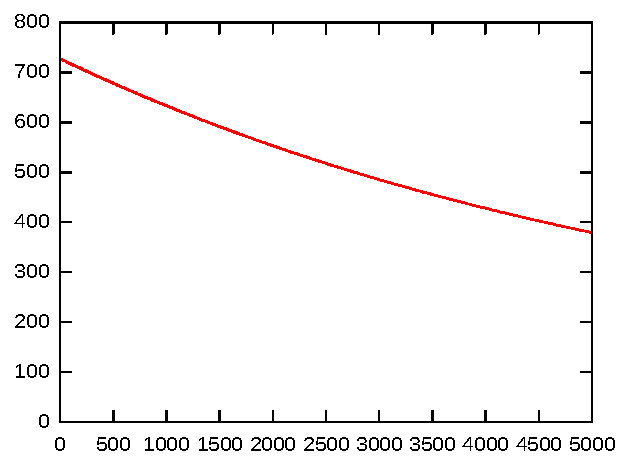
\includegraphics[width=\textwidth]{img/eta-batch-low.pdf}
        \caption{premala stopa učenja}
    \end{subfigure}
    \hfill
    \begin{subfigure}[b]{0.32\textwidth}
        \centering
        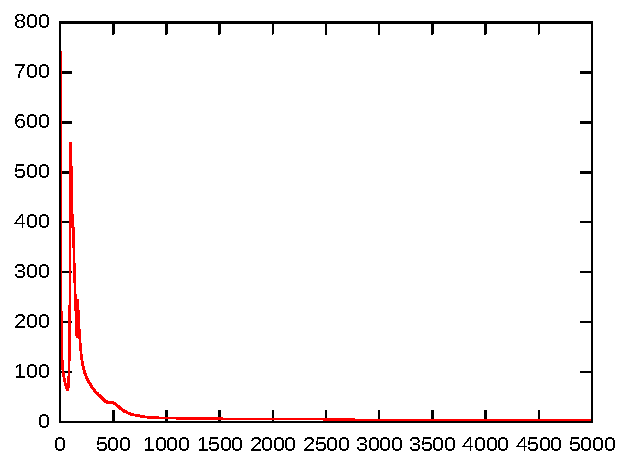
\includegraphics[width=\textwidth]{img/eta-batch-middle.pdf}
        \caption{prikladna stopa učenja}
    \end{subfigure}
    \hfill
    \begin{subfigure}[b]{0.32\textwidth}
        \centering
        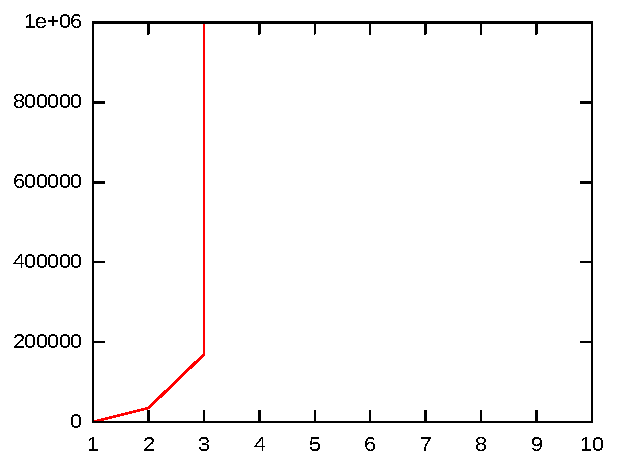
\includegraphics[width=\textwidth]{img/eta-batch-high.pdf}
        \caption{prevelika stopa učenja}
    \end{subfigure}
    \hfill
    \caption{Kretanje srednje pogreške u sustavu s pet pravila - grupni postupak}
    \label{eta-batch}
\end{figure}

\begin{figure}[h]
    \centering
    \begin{subfigure}[b]{0.32\textwidth}
        \centering
        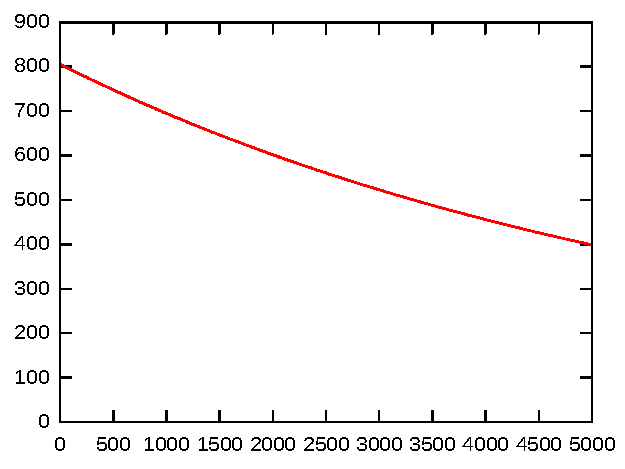
\includegraphics[width=\textwidth]{img/eta-stochastic-low.pdf}
        \caption{premala stopa učenja}
    \end{subfigure}
    \hfill
    \begin{subfigure}[b]{0.32\textwidth}
        \centering
        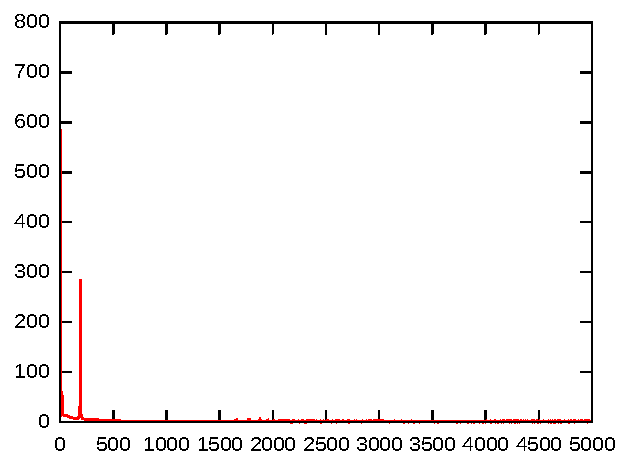
\includegraphics[width=\textwidth]{img/eta-stochastic-middle.pdf}
        \caption{prikladna stopa učenja}
    \end{subfigure}
    \hfill
    \begin{subfigure}[b]{0.32\textwidth}
        \centering
        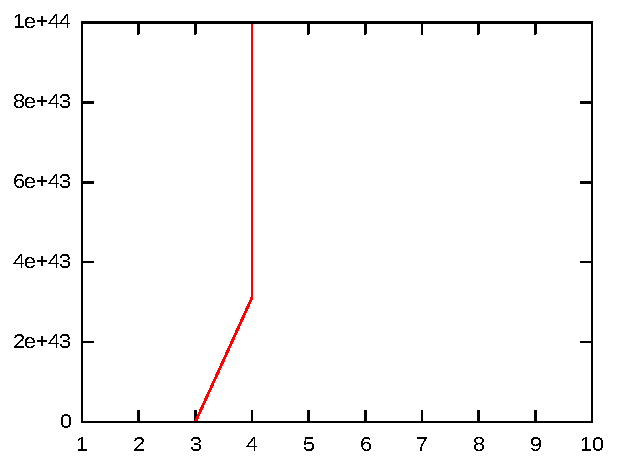
\includegraphics[width=\textwidth]{img/eta-stochastic-high.pdf}
        \caption{prevelika stopa učenja}
    \end{subfigure}
    \hfill
    \caption{Kretanje srednje pogreške u sustavu s pet pravila - stohastički postupak}
    \label{eta-stochastic}
\end{figure}

\end{document}